\documentclass[10pt,a4paper]{article}
\usepackage[latin1]{inputenc}
\usepackage{amsmath}
\usepackage{amsfonts}
\usepackage{amssymb}
\usepackage{graphicx}
\author{Cano Jones, Alejandro}
\title{hiperbola}
\usepackage{pgfplots}
\usepackage{tikz}

\begin{document}
	\pgfplotsset{every axis/.append style={
			axis x line=middle,    % put the x axis in the middle
			axis y line=middle,    % put the y axis in the middle
			axis line style={->}, % arrows on the axis
			xlabel={$x$},          % default put x on x-axis
			ylabel={$y$},          % default put y on y-axis
	}}
\begin{center}
		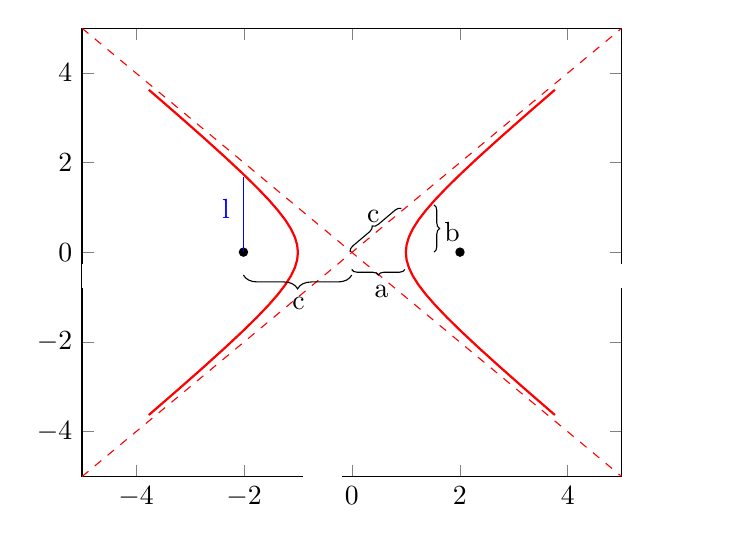
\begin{tikzpicture}
	\begin{axis}[
	xmin=-5,xmax=5,
	ymin=-5,ymax=5]
	\addplot [red,thick,domain=-2:2] ({cosh(x)}, {sinh(x)});
	\addplot [red,thick,domain=-2:2] ({-cosh(x)}, {sinh(x)});
	\addplot[red,dashed] expression {x};
	\addplot[red,dashed] expression {-x};
	\end{axis}
	\fill[white] (3,3.2) rectangle (3.3,5.5);
	\fill[white] (2.8,0) rectangle (3.3,2);
	\fill[white] (0,2.7) rectangle (2.3,2.4);
	\fill[white] (4.5,2.7) rectangle (8,2.4);
	\fill [black] (2.05,2.85) circle (0.06cm);
	\fill [black] (4.8,2.85) circle (0.06cm);
	\draw [decorate,decoration={brace,amplitude=5pt,mirror,raise=4pt},yshift=0pt]
	(2.05,2.7)--(3.425,2.7);
	\draw [decorate,decoration={brace,amplitude=2pt,mirror,raise=2pt},yshift=0pt]
	(3.425,2.7)--(4.1,2.7);
	\draw [decorate,decoration={brace,amplitude=2pt,mirror,raise=2pt},yshift=0pt]
	(4.1,3.35)--(3.45,2.8);
	\draw [decorate,decoration={brace,amplitude=2pt,mirror,raise=2pt},yshift=0pt]
	(4.4,2.85)--(4.4,3.45);
	\draw [blue] (2.05,2.85)--(2.05,3.8);
	\node[blue, left]at(2,3.4){l};
	\node[below]at(2.75,2.4){c};
	\node[below]at(3.8,2.55){a};
	\node[below]at(3.7,3.5){c};
	\node[below]at(4.7,3.35){b};
	\end{tikzpicture}
\end{center}
\end{document}